\documentclass[a4paper,11pt]{article}
\usepackage{amsmath}
\usepackage{xcolor}
\usepackage{soul}
\usepackage{graphicx}
\usepackage{geometry}
\usepackage{float}
\usepackage{hyperref}

\usepackage[labelfont=bf,skip=0pt]{subcaption}
\usepackage[labelfont=bf,skip=0pt]{caption}
\DeclareCaptionFormat{myformat}{\fontsize{8}{8}\selectfont#1#2#3}
\captionsetup{format=myformat}

\newcommand{\hlc}[2][yellow]{{%
    \colorlet{foo}{#1}%
    \sethlcolor{foo}\hl{#2}}%
}

\usepackage{titling}
\setlength{\droptitle}{-2cm}
\title{CombiFF}
\author{Marina P. Oliveira, Salom\'e Rieder, Philippe H. Hünenberger}
\date{}

\geometry{verbose,a4paper,tmargin=20mm,bmargin=20mm,lmargin=15mm,rmargin=15mm}

\begin{document}
\pagestyle{plain}
\maketitle

%================================================================================
\section{\texttt{CombiFF} Workflow}
%================================================================================

The \texttt{CombiFF} workflow is illustrated in Figure \ref{cff_workflow}
%
\begin{figure}[h!]
\begin{center}
  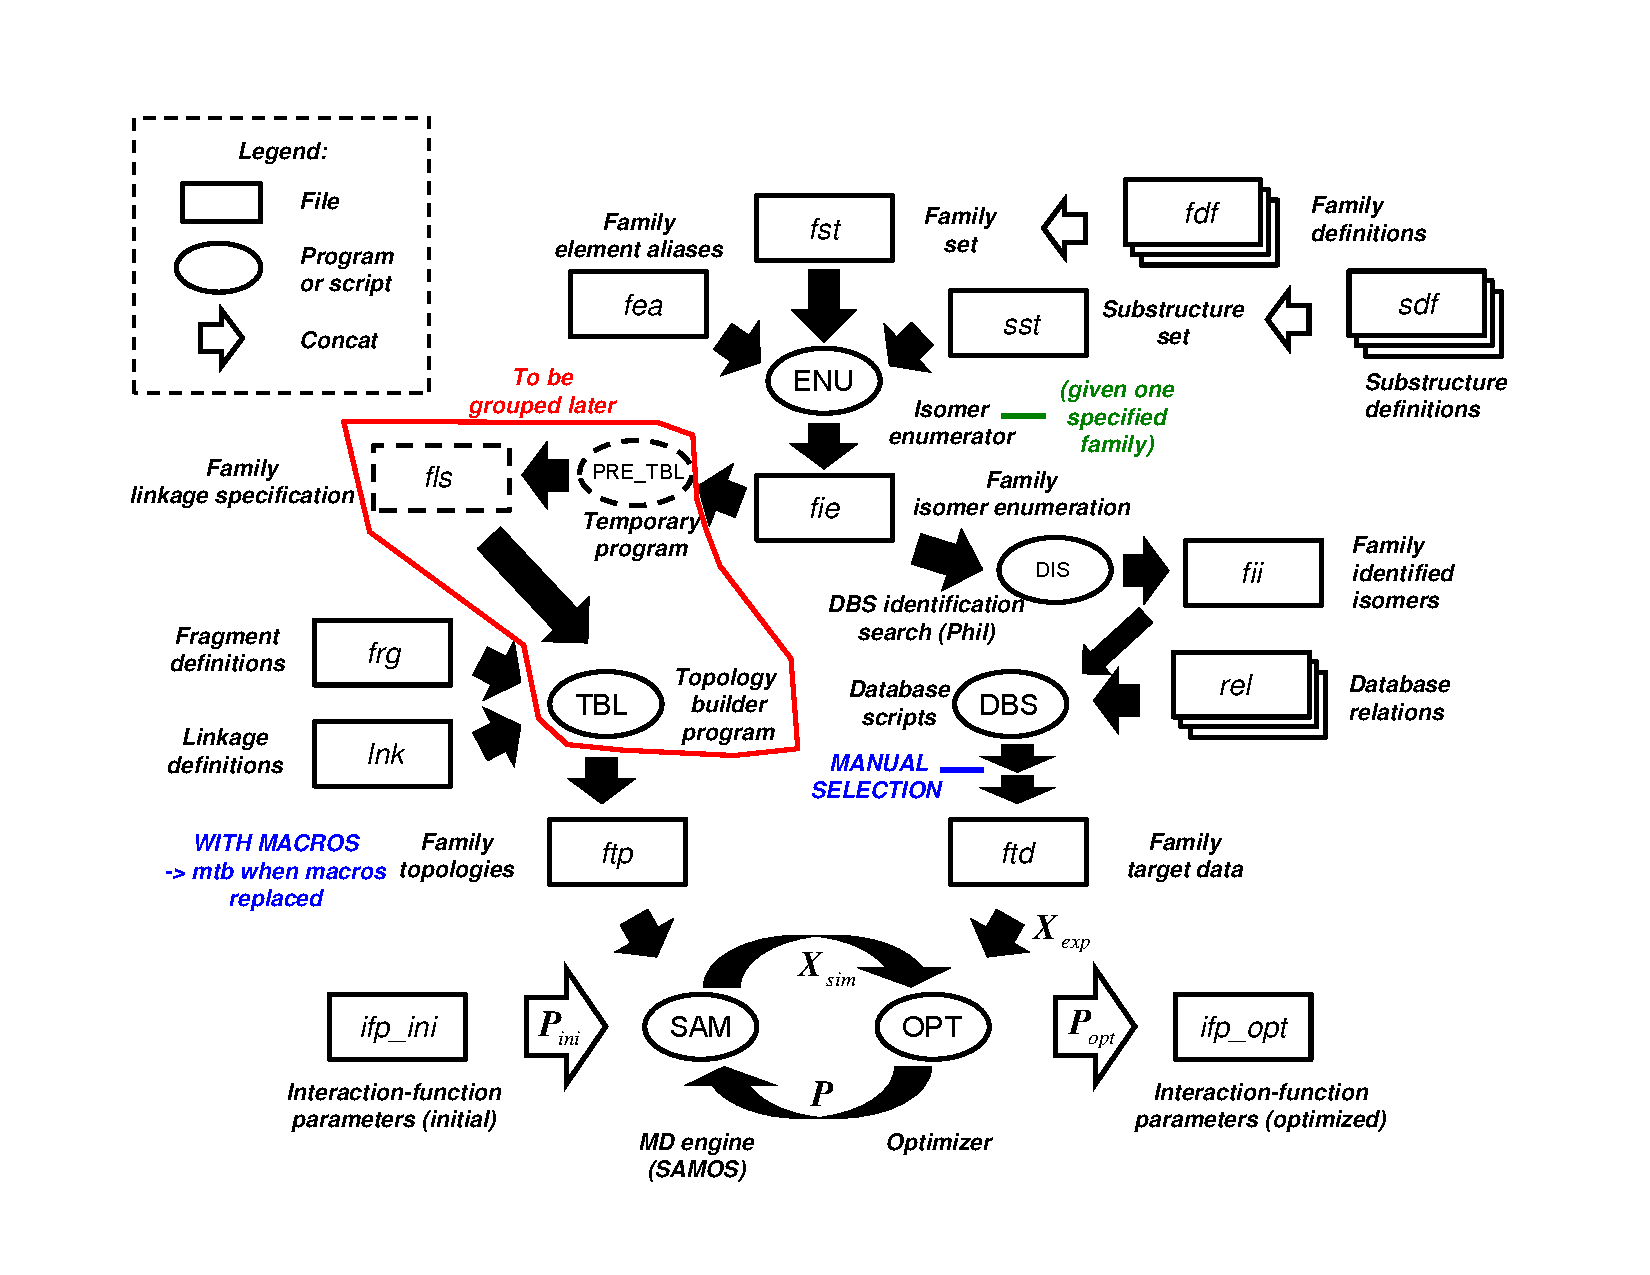
\includegraphics[clip=true,scale=0.6]{fig/cff_workflow.pdf}
\end{center}
\caption{XXX}
\label{cff_workflow}
\end{figure}
%
%



\end{document}



